% !TEX root = ../../../main.tex
% 来源：中学数学实验教材·第三册（高中数学）
% 章节：三角函数的图象和性质 / 正弦型曲线
% 原始文件：7.tex，行 1553-1585
% 类型：tikz
% ---
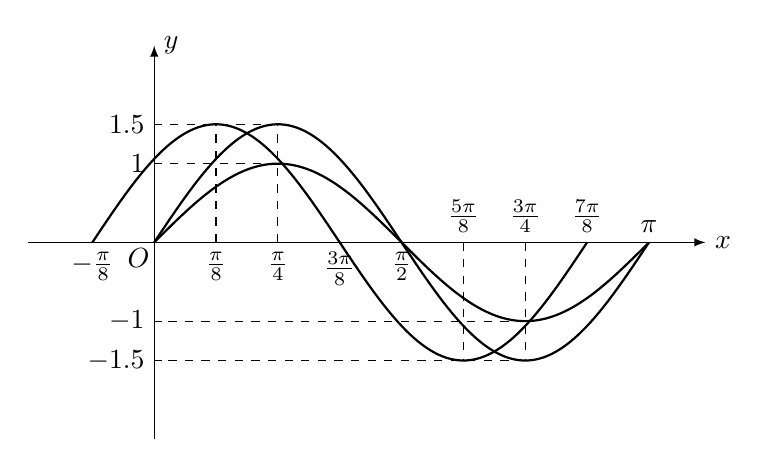
\begin{tikzpicture}[>=latex, xscale=2]
\draw[->](-.8,0)--(3.5,0)node[right]{$x$};
\draw[->] (0,-2.5)--(0,2.5)node[right]{$y$};    

\draw [domain=0:pi, samples=1000, thick] plot(\x, {sin(2*\x  r)});
\draw [domain=0:pi, samples=1000, thick] plot(\x, {1.5*sin(2*\x  r)});
\draw [domain=-pi/8:pi*7/8, samples=1000, thick] plot(\x, {1.5*sin(2*\x r +pi/4  r)});
\node at (-.1,-.2){$O$};

\foreach \x/\xtext in {-1/-\frac{\pi}{8},1/\frac{\pi}{8},2/\frac{\pi}{4},3/\frac{3\pi}{8},4/\frac{\pi}{2}}
{
    \node at (\x*pi/8,0)[below]{$\xtext$};
}

\foreach \x/\xtext in {5/\frac{5\pi}{8},6/\frac{3\pi}{4},7/\frac{7\pi}{8},8/\pi}
{
    \node at (\x*pi/8,0)[above]{$\xtext$};
}

\foreach \x in {1,2}
{
    \draw[dashed] (\x*pi/8,0)--(\x*pi/8,1.5);
    \draw[dashed] (\x*pi/8+0.5*pi,0)--(\x*pi/8+0.5*pi,-1.5);
}

\draw[dashed](pi/4,1.5)--(0,1.5);  \draw[dashed](pi/4,1)--(0,1);
\draw[dashed](3*pi/4,-1.5)--(0,-1.5);  \draw[dashed](3*pi/4,-1)--(0,-1);

\foreach \x in {-1.5,-1,1,1.5}
{
    \draw (0,\x)node[left]{$\x$}--(.05,\x);
}
\end{tikzpicture}
